\documentclass[12pt,a4paper]{article}

\usepackage[letterpaper]{geometry}
\usepackage{times}
\geometry{top=1.0in, bottom=1.5in, left=1.0in, right=1.0in}

\usepackage{fancyhdr}
\pagestyle{fancy}
\lhead{}
\rhead{}
\lfoot{}
\rfoot{}

\renewcommand{\headrulewidth}{0pt} 
\renewcommand{\footrulewidth}{0pt} 

\setlength\headsep{0.333in}

\usepackage{fontspec}
\usepackage{graphicx}
\usepackage{hyperref}
\usepackage{caption}
\usepackage{indentfirst}
\usepackage{setspace}
\usepackage{float}
\usepackage{enumitem}
\usepackage{listings}
\usepackage{color}
\usepackage{xcolor}
\usepackage{tabularx}
\usepackage{amsmath}
\usepackage{siunitx}

\newcommand{\e}[1]{\times10^{#1}}
\newcommand{\degree}{^\circ}

\begin{document}

\begin{titlepage}
\begin{center}
\vspace*{2cm}

\doublespacing
\rule{\linewidth}{0.3mm}

\textsc{
	\large
	UM-SJTU Joint Institute\\ 
	Physical Laboratory\\
	VP141
}

\rule{\linewidth}{0.3mm}


\vspace*{3.5cm}

{
\Large
\textsc{Laboratory Report}\\
}

\vspace*{0.2cm}

{
\large
\textsc{Exercise 4} \\
\textsc{Measurement of the Speed of Sound}
}

\end{center}

\vfill
\normalsize

\hspace*{1cm}
\begin{minipage}{0.4\textwidth}
\begin{tabular}{p{1.7cm}p{4cm}llll}
Name: &  Ren Wang \hspace*{0.6cm} {\fontspec{Hei}\selectfont 王韧} & ID: & 516370910177 & Group: & 11 \\
Name: &  Biyang Guo {\fontspec{Hei}\selectfont 郭铋扬} & ID: & 516370910246 & Group: & 11 \\
\multicolumn{6}{l}{Date: \today}
\end{tabular}
\end{minipage}

\end{titlepage}
\newpage

\onehalfspacing
\tableofcontents

\section{Introduction}

The objective of the exercise is to study several methods of measuring the
speed of sound in air: the resonance method, the phase comparison method, and
the time difference method, including successive difference method in
measurement data processing.
    
Sound is a mechanical wave that propagates through a compressible medium.
It's a longitudinal wave since the direction of vibrations of the medium is
the same as the direction of propagation. Sound with the frequency higher
than $20,000\ Hz$ is called \emph{ultrasound}, which is chosen as the signal
source in this experiment because its wavelength is short enough to measure
the speed precisely.
    
The phase speed $v$, the frequency $f$ and the length $\lambda$ of a wave are
related by the formula 
\begin{equation}\label{vlf}
    v=\lambda f.
\end{equation}

For motion with constant speed $v$ along a straight line, we have 
\begin{equation}\label{vlt}
    v=\frac{L}{t},
\end{equation}
where $L$ is the distance travelled over time $t$. 


\section{Experiment Setup}

The BG-2 Pohl resonator consists of two main parts: a vibrometer and a control
box. The vibrometer is shown in Figure 2. A copper balance wheel is mounted on a
supporting frame, and the axis of the balance wheel is attached to the
supporting frame with a scroll spring. The spring provides an elastic restoring
torque to the wheel, which makes the balance wheel rotating about an equilibrium
position. 

\begin{figure}[H]
\centering
\includegraphics[width=0.9\textwidth]{fig/es1}
\caption{The dependence of the amplitude (left) and phase shift (right) of
  steady-state driven oscillations}
\label{aps} 
\end{figure}

There are many notches on the edge of the balance wheel with one notch being
much deeper than the others. A photoelectric detector is set above the deep
notch. The detector is used to measure the amplitude and the period of
oscillations, and it is connected to the electronic control box. 

A pair of coils is placed at the bottom of the supporting frame, with the
balance wheel fitting exactly into the gap between the two coils. Due to
electromagnetic induction, the wheel will be acted upon an electromagnetic
damping force when the coils are carrying current, and the magnitude of the
damping force can be controlled by changing the current. 

The device is equipped with a motor with an electric wheel and a rod used to
drive the wheel. There is a Period Selection switch and a Period of Driving
Force knob on the electric control box, which allow to control the speed of the
motor precisely. Another photoelectric detector is set above the turntable and
connected to the control box to measure the period of driving force. 

The phase shift can be measured using the glass turntable with an angle scale
and a strobe light. The strobe is controlled by the photoelectric detector above
the wheel. When the deep notch passes the equilibrium position, the detector
sends a signal and the strobe flashes. In a steady state, a line on the angle
scale will be highlighted by the flash of the strobe and the phase difference
can be read from the angle scale directly. 

The amplitude of oscillations is measured by counting the notches on the wheel,
and this measurement is performed by a photoelectric detector with the result
displayed on the electronic control box. 

\begin{figure}[H]
\centering
\includegraphics[width=0.9\textwidth]{fig/es2}
\caption{Vibrometer}\label{vib}
\end{figure}

The function Amplitude Display shows the oscillation amplitude of the balance
wheel and Period Display shows the oscillation period in two modes. When the
Period Selection switch is at position "1", a single oscillation period will be
displayed; when the Period Selection switch is at "10", the time of 10
oscillation periods will be displayed. The reset button works only when the
Period Selection button is at "10".  
    
The period of the driving force can be changed precisely by using the Period of
the driving force knob, but please pay attention that the scale on the knob is
not very accurate. 

The Damping Selection knob changes the damping force by adjusting the electric
current through the coils at the bottom of the wheel. There are six options,
ranging from "0" (no current) to "5" (current of about 0.6 A). Here we use "2",
"3" or "4". 

The strobe generates a flash that allows you to read the phase difference from
the angle scale directly. To protect the strobe, you should turn on the Strobe
switch only when measuring the phase difference. 

The Motor Switch is used to control the motor. You should turn the motor off
when measuring the damping coefficient and the natural angular frequency. 

\begin{figure}[H]
\centering
\includegraphics[width=0.8\textwidth]{fig/es3}
\caption{The front panel of the control box}\label{panel}
\end{figure}

\subsection{Devices precision}
The precisions of the devices are shown in Table \ref{precision}.
\begin{table}[H]
\centering
\begin{tabular}{|l|c|c|}
\hline
Devices & Precision & Unit\\ \hline
Timer on BG-2 Pohl resonator & 0.001 & [s]\\ \hline
Angle on BG-2 Pohl resonator & 1 & [$\degree$]\\ \hline
\end{tabular}
\caption{Devices precision}\label{precision}
\end{table}
\section{Measurement Procedue}

\setenumerate[2]{label=(\arabic*)}

\subsection{Spring constant}

\begin{enumerate}
\item Adjust the Jolly balance to vertical and attach the spring Add a 20g
  preload and adjust knob $I_1$ and $I_2$ to make sure the mirror can move
  freely through the tube. Check if the balance parallel to the spring. 
\item Adjust knob $G$ to make the three lines in the tube coincide.
\item Reading the reading on the scale, add mass from 1 to 6 and record $L_i$ in
  order. 
\item Estimate the spring constant $k_1$ by fitting.
\item Repeat the measurements with spring 2. Calculate $k_2$.
\item Remove the preload and repeat the measurements for spring 1 and 2
  connected. Calculate $k_3$. 
\end{enumerate}

\subsection{Relation between oscillation period $T$ and the mass of the
  oscillator $M$} 

\begin{enumerate}
\item Adjust the air track so that it's horizontal.

\begin{enumerate}
\item Turn on the air track and check whether there's blocked holes.
\item Place the cart on the track. Adjust the track with the knob on the side
  with a single one. 
\end{enumerate}

\item Horizontal air track

\begin{enumerate}
\item Attach springs to the sides of the cart and set up the I-shape shutter.
  Make sure that the photoelectric gate is at the equilibrium position. 
\item Set the timer into "T" mode. Add weight in order and release it with a
  caliper. Record the corresponding time intervals for 10 periods. 
\item Analyze the relation between $M$ and $T$ by plotting a graph. 
\end{enumerate}

\item Inclined air track

\begin{enumerate}
\item Add three plastic plates under the air track every time. Repeat the steps
  in 2. 
\item Analyze the relation between $M$ and $T$ by plotting a graph.
\end{enumerate}

\end{enumerate}

\subsection{Relation between the oscillation period and the amplitude} 

\begin{enumerate}

\item Keep the mass of the cart unchanged and change the amplitude (choose 6
  different values). The amplitude is about 5.0/ 10.0/ 15.0/ ... /30.0 cm. 
\item Apply linear fit to the data and comment on the relation between the
  oscillation period $T$ and the amplitude $A$ based on the correlation
  coefficient $\gamma$. 
\end{enumerate}

\subsection{Relation between the maximum speed and the amplitude}

\begin{enumerate}
\item Keep the mass of the cart unchanged and change the amplitude from $5.0\
  to\ 30.0 cm$ with gap of $5.0cm$. 
\item Measure $v_{max}$ for different amplitudes.
\end{enumerate}

\subsection{Mass measurement}

\begin{enumerate}
\item Adjust the electronic balance every time before you use it. The level
  bubble should be in the center of the circle. 
\item Add weights according to a fixed order. Weigh the cart with the I-shape
  shutter and with the U-shape shutter. Measure the mass of spring 1 and spring
  2. 
\item Record the data only after the circular symbol on the scales display
  disappears. 
\end{enumerate}


\section{Caution}

\begin{itemize}
\item Do not stretch the spring over its elastic limit, otherwise the spring
  will not return to its original shape.  
\item When using the Jolly balance, the mirror should be moving freely in the
  glass tube without any friction. When adding weight, hold the tray steady to
  avoid errors due to vibrations. 
\item Please use tweezers to move the weights around.
\item  Make sure that no air holes on the air tracks are blocked.
\item Avoid scratching the cart. Do not move the cart when pressed against the
  air track.
\end{itemize}

\section{Result}

\section{Results}

\subsection{Measurement for natural angular frequency}
We calculate the angular frequency from Table~\ref{data_omega} by the formula
\[
\omega_0=\frac{2\pi}{T}.
\]
\begin{table}[H] 
\centering
\begin{tabular}{|c|c|}
\hline
& $10T[s] \pm 0.001[s]$\\\hline
1 & 15.790  \\\hline
2 & 15.801  \\\hline
3 & 15.778  \\\hline
4 & 15.800  \\\hline
\end{tabular}
\caption{Measurement of ten periods for the natural frequency}
\label{data_omega}
\end{table}

Hence the average value of $10T$ should be calculated as

\[
\overline{10T}=\frac{1}{4}\sum_{i=1}^{4}(10T)_i=15.79225 \pm 0.0107 \ s, \quad
u_{10T,r}=0.07\%. 
\]

The value of $\omega_0$ is

\[
\overline{\omega_0}=\frac{20\pi}{10T}=\frac{20\times3.1416}{15.79225}= 3.9787
\pm 0.006 \  rad/s,\quad u_{\omega_0,r}=0.15\%. 
\]

\subsection{Measurement for damping coefficient}

The damping coefficient can be calculated by the following formula.

\[
\beta=\frac{1}{5T}\ln\frac{\theta_i}{\theta_{i+5}}.
\]


In the experiment, we choose Damping Selection 2.

\begin{table}[H] 
\centering

\begin{tabular}{|c|c|c|c|c|}
\hline

\multicolumn{2}{|c}{Amplitude[$\degree$]$\pm$1[$\degree$]} & 
\multicolumn{2}{|c|}{Amplitude[$\degree$]$\pm$1[$\degree$]} &
$\ln(\theta_i/\theta_{i+5})$\\\hline

$\theta_0$ & 149 & $\theta_5$ & 95 & 0.4501 \\\hline
$\theta_1$ & 136 & $\theta_6$ & 86 & 0.4583 \\\hline
$\theta_2$ & 124 & $\theta_7$ & 79 & 0.4508 \\\hline
$\theta_3$ & 114 & $\theta_8$ & 72 & 0.4595 \\\hline
$\theta_4$ & 103 & $\theta_9$ & 65 & 0.4603 \\\hline
\multicolumn{4}{|c|}{The average value of $\ln(\theta_i/\theta_{i+5})$}
    & 0.4558 \\\hline 
\end{tabular}

\caption{Measurement of the damping coefficient for Damping Selection 2}
\label{data_damping}
\end{table}

The experimental value of $\ln(\theta_i/\theta_{i+5})$ is shown below

\[
\ln(\theta_i/\theta_{i+5})= 0.4558 \pm 0.0050 , \quad u_r=1.09\%
\]

Here, $T= 15.79225 /10= 1.5792 \pm 0.0001s$. Then we can easily obtain $\beta$
as well, 

\[
\beta=\frac{1}{5\times1.5792}\times0.4558=  0.0577 \pm 0.003s^{-1}, \quad
u_{\beta,r}=5.2\% 
\]

\subsection{Measurement for $\theta_{st}$ vs. $\omega$ and $\varphi$ vs.
  $\omega$}  

To study the relation between $\varphi$ and $\omega/\omega_0$, 

first we get the raw data of 10T, $\phi$ and $\theta$,
we then process the raw data and list them in Table~\ref{data_phi2} and
Table~\ref{data_phi3}. 


\begin{table}[H]
\centering
\begin{tabular}{|c|c|c|c|}
\hline
& $10T [s] \pm 0.001 [s]$ &  $\varphi  [\degree]  \pm 1 [\degree]$ & $ \theta [\degree] \pm 1 [\degree]$ \\ \hline 

1  & 15.098 & -162  &  38   \\ \hline
2  & 15.123 & -163  &  39   \\ \hline
3  & 15.542 & -143  &  87   \\ \hline
4  & 15.672 & -118  &  130  \\ \hline
5  & 15.707 & -109  &  138  \\ \hline
6  & 15.724 & -103  &  141  \\ \hline
7  & 15.736 & -100  &  143  \\ \hline
8  & 15.755 & -94   &  145  \\ \hline
9  & 15.763 & -92   &  146  \\ \hline
10 & 15.774 & -89   &  144  \\ \hline
11 & 15.788 & -86   &  144  \\ \hline
12 & 15.797 & -84   &  144  \\ \hline
13 & 15.810 & -82   &  144  \\ \hline
14 & 15.820 & -79   &  142  \\ \hline
15 & 15.841 & -75   &  140  \\ \hline
16 & 15.907 & -64   &  130  \\ \hline
17 & 15.946 & -57   &  124  \\ \hline
18 & 16.050 & -46   &  105  \\ \hline
19 & 16.131 & -40   &  92   \\ \hline
20 & 16.237 & -33   &  78   \\ \hline
21 & 16.472 & -22   &  54   \\ \hline
22 & 16.603 & -18   &  46   \\ \hline
\end{tabular}    
\caption{$\theta$ vs. $10T$ and $\varphi$ vs. $10T$ raw data for Damping
  selection 2} 
\end{table}

\begin{table}[H]
\centering
\begin{tabular}{|c|c|c|c|}
\hline
& $10T [s] \pm 0.001 [s]$ &  $\varphi  [\degree]  \pm 1 [\degree]$ & $ \theta [\degree] \pm 1 [\degree]$ \\ \hline

1  & 15.057   & -163 &  35   \\ \hline
2  & 15.302   & -155 &  50   \\ \hline
3  & 15.526   & -142 &  79   \\ \hline
4  & 15.657   & -123 &  108  \\ \hline
5  & 15.708   & -111 &  120  \\ \hline
6  & 15.745   & -104 &  125  \\ \hline
7  & 15.760   & -97  &  127  \\ \hline
8  & 15.794   & -93  &  128  \\ \hline
9  & 15.789   & -92  &  128  \\ \hline
10 & 15.803   & -89  &  128  \\ \hline
11 & 15.814   & -86  &  128  \\ \hline
12 & 15.830   & -83  &  128  \\ \hline
13 & 15.849   & -80  &  126  \\ \hline
14 & 15.883   & -74  &  124  \\ \hline
15 & 15.903   & -69  &  120  \\ \hline
16 & 15.933   & -62  &  114  \\ \hline
17 & 16.013   & -55  &  106  \\ \hline
18 & 16.102   & -47  &  93   \\ \hline
19 & 16.168   & -41  &  83   \\ \hline
20 & 16.290   & -33  &  70   \\ \hline
21 & 16.452   & -25  &  55   \\ \hline
22 & 16.585   & -18  &  46   \\ \hline
\end{tabular}    
\caption{$\theta$ vs. $10T$ and $\varphi$ vs. $10T$ raw data for Damping
  selection 3} 
\end{table}


Then We know that $ \omega / \omega_0 = T_0 / T $,
thus we can have the following processed data.


\begin{figure}
  \centering
\begin{minipage}{0.45\textwidth}
\begin{table}[H]
\centering
\begin{tabular}{|c|c|c|}
\hline
& $\omega/\omega_0$ &  $\varphi \pm 1 [\degree] $ \\ \hline
1  & 1.0460  & -162  \\ \hline
2  & 1.0443  & -163  \\ \hline
3  & 1.0161  & -143  \\ \hline
4  & 1.0077  & -118  \\ \hline
5  & 1.0054  & -109  \\ \hline
6  & 1.0043  & -103  \\ \hline
7  & 1.0036  & -100  \\ \hline
8  & 1.0024  & -94   \\ \hline
9  & 1.0019  & -92   \\ \hline
10 & 1.0012  & -89   \\ \hline
11 & 1.0003  & -86   \\ \hline
12 & 0.9997  & -84   \\ \hline
13 & 0.9989  & -82   \\ \hline
14 & 0.9982  & -79   \\ \hline
15 & 0.9969  & -75   \\ \hline
16 & 0.9928  & -64   \\ \hline
17 & 0.9904  & -57   \\ \hline
18 & 0.9839  & -46   \\ \hline
19 & 0.9790  & -40   \\ \hline
20 & 0.9726  & -33   \\ \hline
21 & 0.9587  & -22   \\ \hline
22 & 0.9512  & -18   \\ \hline
\end{tabular}    
\caption{$\varphi$ vs. $\omega/\omega_0$,\\ Damping selection
  2}\label{data_phi2} 
\end{table}
\end{minipage}
%
\begin{minipage}{0.45\textwidth}
\begin{table}[H]
\centering
\begin{tabular}{|c|c|c|}
\hline
& $\omega/\omega_0$ &  $\varphi \pm 1 [\degree] $ \\ \hline
1  & 1.0488   & -163 \\ \hline
2  & 1.0320   & -155 \\ \hline
3  & 1.0171   & -142 \\ \hline
4  & 1.0086   & -123 \\ \hline
5  & 1.0054   & -111 \\ \hline
6  & 1.0030   & -104 \\ \hline
7  & 1.0020   &  -97 \\ \hline
8  & 0.9999   &  -93 \\ \hline
9  & 1.0002   &  -92 \\ \hline
10 & 0.9993   &  -89 \\ \hline
11 & 0.9986   &  -86 \\ \hline
12 & 0.9976   &  -83 \\ \hline
13 & 0.9964   &  -80 \\ \hline
14 & 0.9943   &  -74 \\ \hline
15 & 0.9930   &  -69 \\ \hline
16 & 0.9912   &  -62 \\ \hline
17 & 0.9862   &  -55 \\ \hline
18 & 0.9808   &  -47 \\ \hline
19 & 0.9768   &  -41 \\ \hline
20 & 0.9694   &  -33 \\ \hline
21 & 0.9599   &  -25 \\ \hline
22 & 0.9522   &  -18 \\ \hline
\end{tabular}    
\caption{$\varphi$ vs. $\omega/\omega_0$,\\ Damping selection
  3}\label{data_phi3} 
\end{table}
\end{minipage}
\vspace*{5cm}
\end{figure}

\begin{figure}[H]
\centering
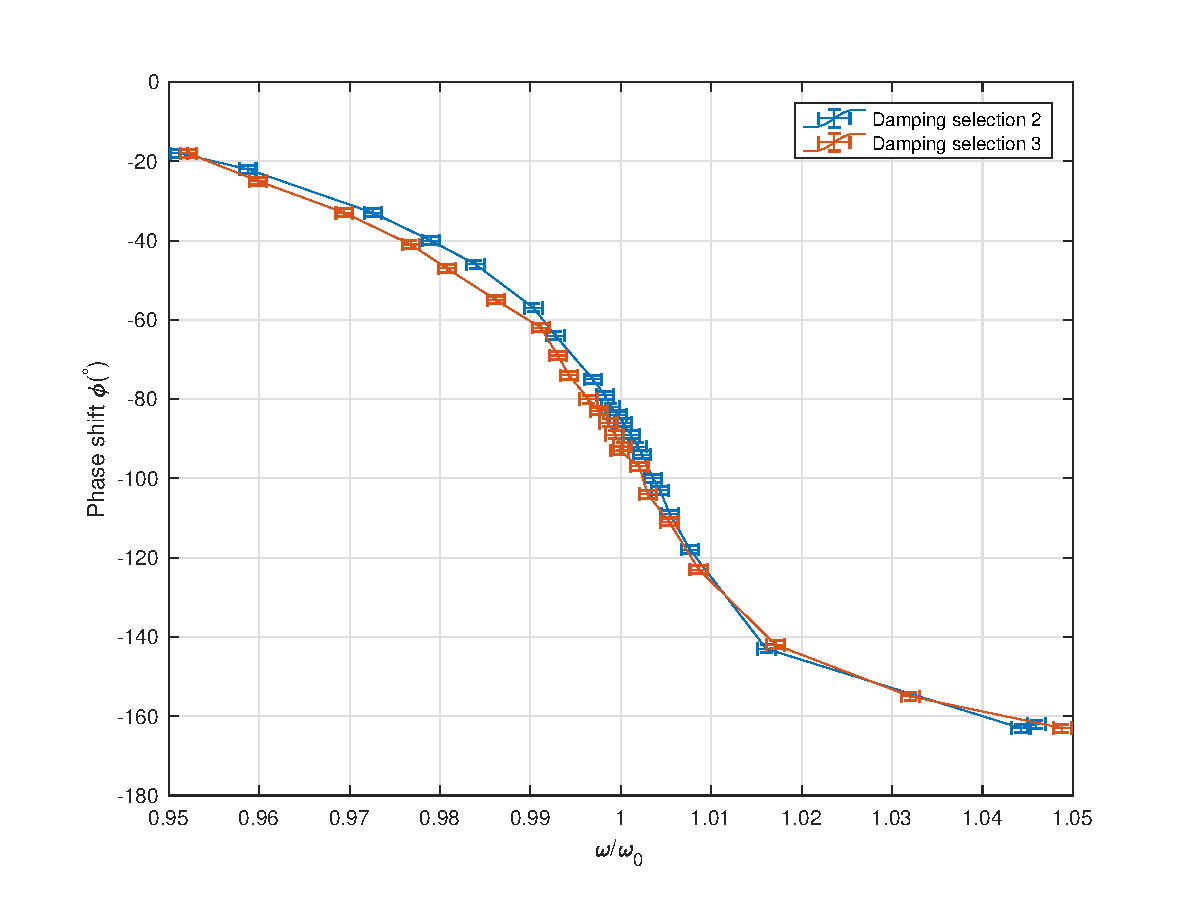
\includegraphics[width=1\textwidth]{matlab/p1}
\caption{Phase shift $\varphi$ vs. $\omega/\omega_0$}\label{phi}
\end{figure}


To study the relation between $\theta_{st}$ and $\omega/\omega_0$, we process the raw data and list them in Table~\ref{data_t2} and Table~\ref{data_t3}.


% TODO:




\begin{figure}
  \centering
\begin{minipage}{0.45\textwidth}
\begin{table}[H]
\centering
\begin{tabular}{|c|c|c|}
\hline
& $\omega/\omega_0$ &  $\theta \pm 1 [\degree] $ \\ \hline
1  & 1.0460  & 38   \\ \hline
2  & 1.0443  & 39   \\ \hline
3  & 1.0161  & 87   \\ \hline
4  & 1.0077  & 130  \\ \hline
5  & 1.0054  & 138  \\ \hline
6  & 1.0043  & 141  \\ \hline
7  & 1.0036  & 143  \\ \hline
8  & 1.0024  & 145  \\ \hline
9  & 1.0019  & 146  \\ \hline
10 & 1.0012  & 144  \\ \hline
11 & 1.0003  & 144  \\ \hline
12 & 0.9997  & 144  \\ \hline
13 & 0.9989  & 144  \\ \hline
14 & 0.9982  & 142  \\ \hline
15 & 0.9969  & 140  \\ \hline
16 & 0.9928  & 130  \\ \hline
17 & 0.9904  & 124  \\ \hline
18 & 0.9839  & 105  \\ \hline
19 & 0.9790  & 92   \\ \hline
20 & 0.9726  & 78   \\ \hline
21 & 0.9587  & 54   \\ \hline
22 & 0.9512  & 46   \\ \hline
\end{tabular}    
\caption{$\theta$ vs. $\omega/\omega_0$,\\ Damping selection 2}\label{data_t2}
\end{table}
\end{minipage}
%
\begin{minipage}{0.45\textwidth}
\begin{table}[H]
\centering
\begin{tabular}{|c|c|c|}
\hline
& $\omega/\omega_0$ &  $\theta \pm 1 [\degree] $ \\ \hline
1  & 1.0488   & 35   \\ \hline
2  & 1.0320   & 50   \\ \hline
3  & 1.0171   & 79   \\ \hline
4  & 1.0086   & 108  \\ \hline
5  & 1.0054   & 120  \\ \hline
6  & 1.0030   & 125  \\ \hline
7  & 1.0020   & 127  \\ \hline
8  & 0.9999   & 128  \\ \hline
9  & 1.0002   & 128  \\ \hline
10 & 0.9993   & 128  \\ \hline
11 & 0.9986   & 128  \\ \hline
12 & 0.9976   & 128  \\ \hline
13 & 0.9964   & 126  \\ \hline
14 & 0.9943   & 124  \\ \hline
15 & 0.9930   & 120  \\ \hline
16 & 0.9912   & 114  \\ \hline
17 & 0.9862   & 106  \\ \hline
18 & 0.9808   & 93   \\ \hline
19 & 0.9768   & 83   \\ \hline
20 & 0.9694   & 70   \\ \hline
21 & 0.9599   & 55   \\ \hline
22 & 0.9522   & 46   \\ \hline
\end{tabular}    
\caption{$\theta$ vs. $\omega/\omega_0$,\\ Damping selection 3}\label{data_t3}
\end{table}
\end{minipage}
\vspace*{5cm}
\end{figure}

\begin{figure}[H]
\centering
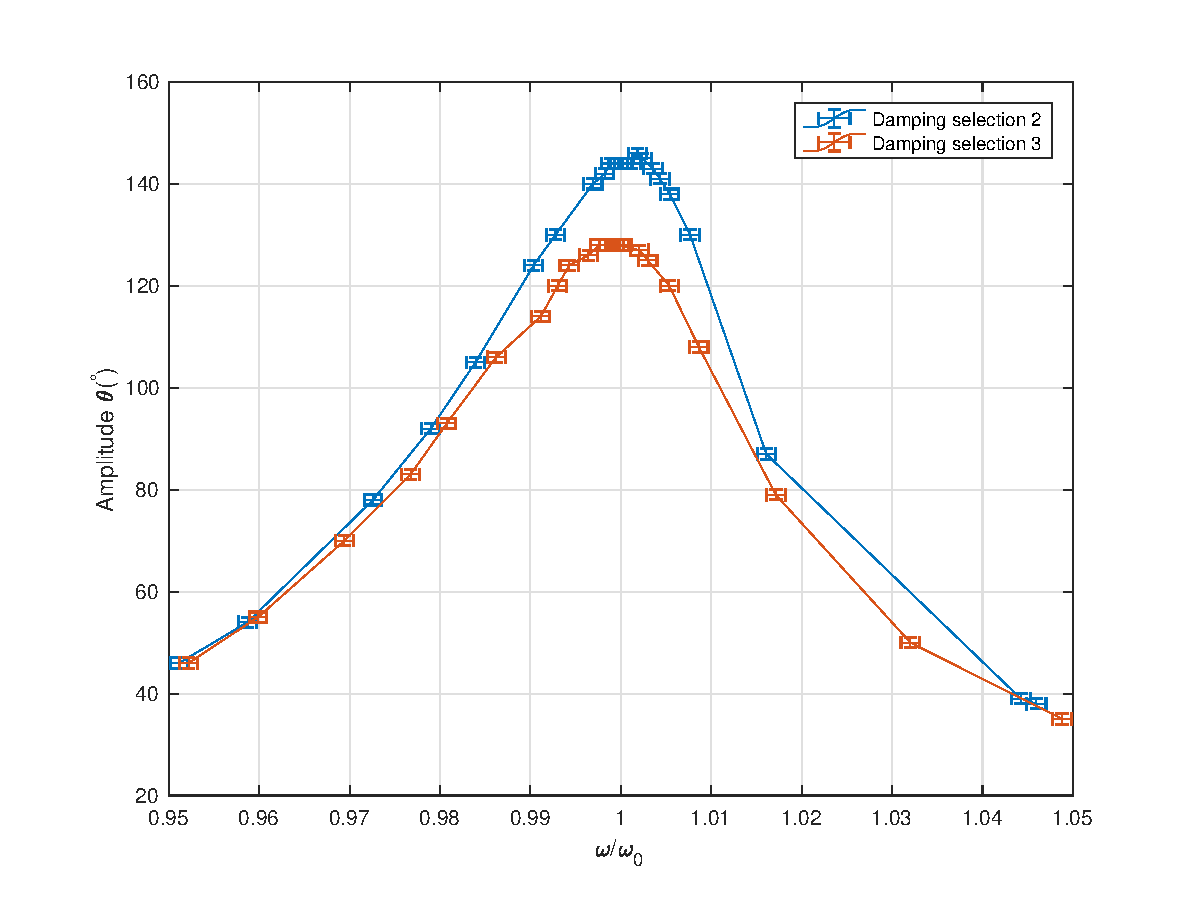
\includegraphics[width=1\textwidth]{matlab/p2}
\caption{Amplitude $\theta_{st}$ vs. $\omega/\omega_0$}\label{theta}
\end{figure}
\section{Measurement Uncertainty Analysis}

\subsection{Uncertainty for natural angular frequency}

To estimate type-A uncertainty of $(10T)$,
the standard deviation of the average value can be calculated as

\[
\begin{split}
&t_{0.95}=3.18,\quad n=4,\\
&s_{\overline{10T}}=\sqrt{\frac{1}{n(n-1)}\sum_{i=1}^n((10T)_i-\overline{10T})^2}.\\ 
&\Delta_{10T,A}=\frac{3.18}{\sqrt{4}}\times0.0076811\approx 0.017s.
\end{split}
\]

The type-B uncertainty of $(10T)$ is 0.001s. Hence, the uncertainty of $(10T)$ is

$$ u_{10T}=\sqrt{\Delta_A^2+\Delta_B^2}=\sqrt{0.017^2+0.001^2}\approx 0.017s $$  

For the uncertainty of $\omega_0$,

$$\omega_0=\frac{20\pi}{10T},\quad \frac{\partial \omega_0}{\partial
  (10T)}=-\frac{20\pi}{(10T)^2}$$ 

\[
\begin{split}
&u_{\omega_0}=\sqrt{\frac{\partial \omega_0}{\partial
    (10T)}^2(u_{10T})^2}=\frac{20\pi}{(10T)^2}u_{(10T)}\\
&=\frac{20\times3.1416}{15.485^2} \times 0.017 = 0.004rad/s,\\  
\end{split}
\]

$$ u_{\omega_0,r}=\frac{u_{\omega_0}}{\omega_0}\times100\%
=\frac{0.004}{4.058}=0.10\% $$ 

\subsection{Uncertainty of damping coefficient}

The type-A uncertainty of $\ln(\theta_i/\theta_{i+5})$ can be determined by
calculating $s\times t_{0.95}/\sqrt{n}$.

Let $k = s \times t_{0.95}/\sqrt{n}$.


$$ t_{0.95}=2.78,\quad n=5$$ 

$$ \Delta_{A,k}=t_{0.95}/\sqrt{5}\times
\sqrt{\frac{1}{5-1}\sum_{i=1}^5(k_i-\bar{k})^2}=2.78/\sqrt{5}\times
0.00444 = 0.005 $$ 

Then, for the type-B uncertainty, 

$$ \frac{\partial k}{\partial \theta_{i}}=\frac{1}{\theta_i} $$
$$ \frac{\partial k}{\partial \theta_{i+5}}=-\frac{1}{\theta_{i+5}} $$ 
$$ \Delta_{B,k}=\sqrt{\frac{\partial k}{\partial
    \theta_{i}}^2(u_{\theta_i})^2+\frac{\partial k}{\partial
    \theta_{i+5}}^2(u_{\theta_{i+5}})^2}
=\sqrt{(\frac{u_{\theta_i}}{\theta_i})^2+(\frac{u_{\theta_{i+5}}}{\theta_{i+5}})^2}  $$ 


When $i=0$, $\theta_0=89\degree$, $u_{\theta_2}=1\degree$,
$\theta_5=54\degree$, $u_{\theta_5}=1\degree$. 

\[
\Delta_{B,k}=\sqrt{(\frac{1}{89})^2+(\frac{1}{54})^2}=0.022 
\]

Considering the type-B uncertainty of $\ln(\theta_i/\theta_{i+5})$, the combined
uncertainty is 

\[
\begin{split}
u_{k}&=\sqrt{(0.005)^2+(0.022)^2}= 0.022,\\
u_{k,r}&=\frac{u_k}{\bar{k}}\times100\%=\frac{0.022}{0.511}\times100\%=4\%
\end{split}
\]

Hence

$$ \ln(\theta_i/\theta_{i+5})=0.456\pm0.005, \quad u_r=1.09\% $$ 

For $10T=15.792 \pm 0.001s$, we know that
\[
T=1.5792\pm0.0001s, \quad u_{r,T}=0.006\%.
\]

Then calculate the uncertainty of $\beta=\ln(\theta_i/\theta_{i+5})/(5T)$.

$$ \frac{\partial \beta}{\partial T}=-\frac{k}{5T^2}$$ 

$$ \frac{\partial \beta}{\partial k}=\frac{1}{5T} $$

\[
\begin{split}
u_{\beta}&=\sqrt{(\frac{\partial \beta}{\partial T})^2(u_T)^2+(\frac{\partial
    \beta}{\partial k})^2(u_k)^2}  
=\sqrt{(\frac{k^2}{25T^4})(u_T)^2+(\frac{1}{25T^2})(u_k)^2}\\
&=\sqrt{(\frac{0.511^2}{25\times1.5792^4})(0.0001^2)+(\frac{0.022^2}{25\times1.579
    2^2})}  \\ 
&= 0.003s^{-1} 
\end{split}
\]

where $k=\ln(\theta_i/\theta_{i+5})$.

Thus, 

\[
\beta=0.0648\pm 0.003s^{-1}, \quad u_{\beta,r}=5\%
\]


% TODO:

\subsection{Uncertainty of $\theta_{st}$ vs. $\omega$ and $\varphi$ vs. $\omega$}

We denote that $r=\omega/\omega_0$.
To determine the uncertainty of ratio, we know that

$$ r=\frac{20\pi}{10T\omega_0} $$ 
$$ \frac{\partial r}{\partial (10T)}=-\frac{20\pi}{(10T)^2\omega_0} $$ 
$$ \frac{\partial r}{\partial \omega_0}=-\frac{20\pi}{(10T)\omega_0^2} $$

\[
\begin{split}
u_{r}&=\sqrt{(\frac{\partial r}{\partial
    (10T)})^2(u_{10T})^2+(\frac{\partial r}{\partial
    \omega_0})^2(u_{\omega_0})^2}\\ 
&=\sqrt{\frac{400\pi^2}{(10T)^4\omega_0^2}(u_{10T})^2+\frac{400\pi^2}{(10T)^2\omega_0^4}(u_{\omega_0})^2}.
\end{split}
\]

As is calculated before, $\omega_0=3.9787 \pm 0.006 \ rad/s$.

For instance, when $10T= 15.79225  \pm 0.001s$, the uncertainty of $r$ is
\[
u_{r}=\sqrt{\frac{400\times3.1416^2}{15.79225 ^4\times 3.9787^2}(0.001)^2
  +\frac{400\times3.1416^2}{15.79225^2\times3.9787^4}(0.004)^2}=0.0009
\] 

For the uncertainty of $\varphi$ and $\theta$, these two data only obtain type-B
uncertainty, so the combined uncertainty of them are both equal to
$\Delta_B=1\degree$, thus 

$$ u_{\varphi}=1\degree $$
$$ u_{\theta}=1\degree. $$

\section{Conclusion and Discussion}

\subsection{The resonance method and the comparison method}
    In this experiment the spped of sound in the air was found by two means: the resonance method and the phase comparison method. The two results yielded the values
    \begin{equation}\label{res}
    \begin{split}
        v&=351.05\pm0.4 m/s,\quad u_{r,v}=0.10\%;\\
        v&=348.95\pm10 m/s,\quad u_{r,v}=3\%,
    \end{split}
    \end{equation}
    respectively. The resonance method obtains obviously smaller uncertainty. To compare these two experimentally found results, we need an objective standard.

    According to Bohn Dennis A. in the report "Environmental effects on the speed of sound", \emph{Journal of the Audio Engineering Society} P223-231, the speed of sound with respect to temperature holds the following equation
    \[
        c=331.45\sqrt{1+\frac{t}{273}}\quad\quad\quad\quad\cite{foo1},
    \]
    where $c$ is the sound of the speed and $t$ is the temperature in degrees Celsius.

    Since temperature we meausured was $\SI{24\pm1}{\degreeCelsius}$, the "theoretical" value of sound speed should be
    \[
        v=331.45\sqrt{1+\frac{24}{273}}=345.71m/s
    \]
    which is within the uncertainty interval of the results with the phase comparison method.

    Hence we can conclude that the results of the resonance method is \textbf{precise enough} but \textbf{not accurate enough}. 
    
    On the contrary, the results of the phase comparison method is \textbf{accurate enough} but \textbf{not precise enough}.\\

    The possible reason for errors in the resonance method is the system error. Since the uncertainty is quite small, there should exists a certain error between the experimental value and the theoretical value, probably becasue the frequency displayed on the screen had a certain deviation.

    The possible reason for errors in the phase comparison method is the reading error. We found that it was still changing in shape after we stop moving the calliper so that it's hard to tell whether it's the straight segment we want. Besides, the reading of calliper was inaccurate. 

\subsection{The time difference method for $v_{water}$}
    The experimentally found value is
    \[
        v_{water}=1515\pm20m/s,\quad u_{r,v}=1.5\%.
    \]

    According to the experiment results of N Bilaniuk and GSK Wong in the report "Speed of sound in pure water as a function of temperature", 
    \begin{table}[H]
        \centering
        \begin{tabular}{|c|c|c|c|c|c|}
        \hline
            $t(\SI{}{\degreeCelsius})$ & 23.8 & 23.9 & 24.0 & 24.1 & 24.2\\\hline
            $v(m/s)$ & 1493.440 & 1493.717 & 1493.992 & 1494.267 & 1494.541\\\hline
        \end{tabular}
        \caption{Speed of sound in water with respect to temperature\cite{foo2}}\label{water}
    \end{table}

    We find that our experimental value is relatively close to the standard value.

\subsection{Recommendations}
    For the resonance method, I think it'll be more accurate if there exists somthing like a prompting light to prompt the user when the voltage begins decreasing so that the user can stop the calliper in time and read the accurate value of length.
\section{Reference}
\begin{enumerate}
\end{enumerate}
% ===================
\section{Data Sheet}

\end{document}